\documentclass[conference]{IEEEtran}
\usepackage[T1]{fontenc}
\usepackage{mathptmx,amsmath,amssymb,booktabs,array,graphicx,url,balance}
\usepackage[hidelinks]{hyperref}
\hypersetup{pdfauthor={Xiaotong Wu},pdftitle={Matched Conditioning in Layer-Gate BEV: A Bounded Study of Critical Misses},pdfsubject={Exploratory research report; Research Advisor: Dr. Zhiyu Quan}}
\setlength{\emergencystretch}{1.5em}
\title{Matched Conditioning in Layer-Gate BEV:\\A Bounded Study of Critical Misses}
\author{\IEEEauthorblockN{Xiaotong Wu}\IEEEauthorblockA{Illinois Risk Lab (IRisk Lab)\\University of Illinois Urbana-Champaign\\xiaotongwu116@gmail.com\\\textit{Research Advisor: Dr. Zhiyu Quan}}}
\pagestyle{plain}
\begin{document}
\maketitle
\begin{abstract}
Does current-frame conditioning improve critical pedestrian matching beyond an equally sized input-independent gate? We test a bounded residual around an inherited camera/LiDAR mixture in a BEVFormer-derived detector. Dynamic and constant-descriptor gates each have 29,380 parameters and use common feature pooling, inherited checkpoints, data draws, adaptation updates, and a frozen decoder LiDAR route. Twelve fixed trajectories cover two original folds and three seeds on historically exposed nuScenes mini. The 162-frame, four-log outer panel contains 1,347 critical pedestrian observations. Dynamic-minus-constant pedestrian hit changes are $-2,+2,+9$ across the three seeds, or $-0.148,+0.148,+0.668$ percentage points. Exact annotation matching reveals recovery/loss pairs of $5/7,5/3,9/0$; joint-VRU AnyMiss failures change from $131,124,130$ to $131,125,130$ of 137 target-containing frames. All seeds fail the frozen useful-effect screen. Realized coefficients vary across frames, yet none of the primary count-improved frames becomes all-clear. Decoder-input masking, per-log SDK metrics, neutral-parent comparisons, and exact identity turnover delimit interpretation without establishing causal contributions or fresh-data efficacy. The completed finite study supports no stable practical advantage for conditioning under this implementation and budget. It preserves historical failures and provides compact arithmetic reproduction with explicit limits.
\end{abstract}
\begin{IEEEkeywords}bird's-eye view, multimodal fusion, critical misses, conditional gating, reproducibility\end{IEEEkeywords}
\section{Question and prior work}
This follow-up asks whether current-frame conditioning improves critical pedestrian matching beyond an input-independent gate when inherited checkpoints, adaptation updates, module shapes, sampling, and inference paths are matched. It tests a bounded coefficient residual in the existing detector. Limiting departures from its learned static mixture is a design motivation. The falsifiable hypothesis is a conditioning advantage under that declared bound; both arms are bounded, so the experiment cannot establish a benefit of bounding itself. Improvement is not a completion requirement.

The completed predecessor reported mixed gate results and no stable efficacy~\cite{Wu2026CriticalMiss}. In its A2/seed1/clean comparison, pedestrian hits increased from 1,000 to 1,007 of 2,923 observations, while joint-VRU AnyMiss retained the same 288 failed identities among 307 joint-target frames. That saved-count study could not identify which individual annotations changed match status. It already included a same-shape constant-descriptor A3 control. The present direct dynamic--constant comparison tightens common pooling and execution paths under the bounded formula, while saving exact target turnover. Its smaller four-log panel and newly computed outputs are a separate experiment, not a repair or rerun of the earlier matrix, and capacity matching itself is not a new contribution.

BEVFormer builds BEV representations from camera views through spatial cross-attention and historical BEV through temporal self-attention~\cite{Li2022BEVFormer}. Its official transformer passes the encoder BEV embedding to the detection decoder~\cite{BEVFormerCode}. Our current-frame camera/LiDAR customization disables temporal history and adds LiDAR processing, so it is BEVFormer-derived rather than a reproduction of the original system. Conditional modulation and neutral residual initialization are established design ideas: FiLM conditions feature-wise affine transformations~\cite{Perez2018FiLM}, while ReZero introduces initially zero residual weights~\cite{Bachlechner2021ReZero}. Neither provides evidence for this detector's critical-miss behavior. The earlier project gate already had neutral initialization and conditioned outputs; the present changes are the bounded coefficient residual and tighter controls, without a priority claim.

\section{Architecture and gradient paths}
\begin{figure*}[t]
\centering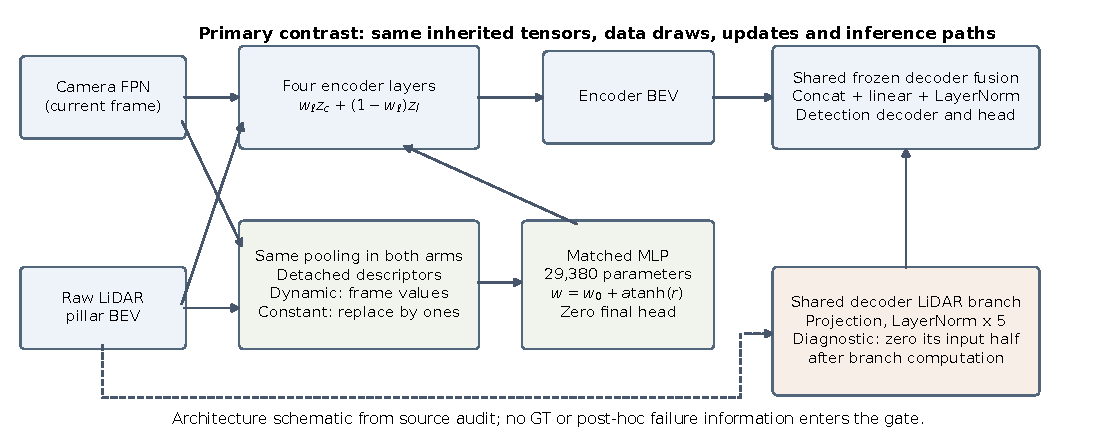
\includegraphics[width=\textwidth]{images/matched_architecture.pdf}
\caption{Matched source-level architecture. Both arms pool the actual current-frame features before retaining dynamic descriptors or replacing them with constants. The shared decoder LiDAR route is frozen; its inference masking is a separate intervention. No annotation or post-hoc failure information enters the gate.}\label{fig:architecture}
\end{figure*}
At each of four encoder layers, a scalar camera coefficient blends camera and projected-LiDAR attention outputs:
\begin{equation}
 z_\ell=w_\ell z_{\ell,c}+(1-w_\ell)z_{\ell,l}.
 \label{eq:blend}
\end{equation}
Coefficients vary by frame and layer but are shared spatially. They are not object-specific masks and receive no annotation, sample identity, prediction, or post-hoc failure information at inference. A frame containing both recovered and missed pedestrians therefore receives a common mixture at each layer; spatially selective recovery is not directly specified by this gate.

In the ordinary nonempty camera-attention branch, both attention outputs include the same query residual. Writing their remaining attention terms as $A_c,A_l$ gives $z=q+wA_c+(1-w)A_l$. The audited customized camera-attention code also has an all-camera-masks-empty fallback returning $\operatorname{dropout}(q)+q$, equal to $2q$ in evaluation for that residual input. That exception prevents treating the ordinary residual simplification as unconditional; its real-data incidence is not measured here. The shared implementation is kept fixed during this contrast; real-data incidence and impact require a separate instrumented evaluation. The general derivative using complete branch outputs remains valid:
\begin{equation}
 \frac{\partial\mathcal L}{\partial r_\ell}
 =a_\ell\operatorname{sech}^{2}(r_\ell)
 \left\langle\frac{\partial\mathcal L}{\partial z_\ell},
 z_{\ell,c}-z_{\ell,l}\right\rangle.
\end{equation}
The inner product sums spatial/channel contributions to one frame-level decision. Object-specific improvements and regressions can compete in that aggregate. The detector loss is not the discontinuous AnyMiss endpoint; observing an active gradient does not imply that the last remaining missed target in a frame will recover.

The audited implementation also routes LiDAR features to the decoder independently of Eq.~\eqref{eq:blend}. A $64\!\rightarrow\!256$ convolution and token-wise LayerNorm, scaled by five, produce the decoder LiDAR representation. It is concatenated with encoder BEV and passed through a $512\!\rightarrow\!256$ linear transformation and LayerNorm. This route is retained identically, with its parameters frozen, in both adaptation arms. The primary contrast estimates incremental conditioning \emph{conditional on this shared route}; it cannot establish gate efficacy in a detector without that route.

The source audit also finds this route in every original A0--A3 arm, under the same encoder--decoder fusion configuration and frozen adaptation guards. Its presence is therefore not, by itself, evidence of a differential architectural confound in those comparisons. The original A0 static control's four trainable logits versus the dynamic module's 29,380 parameters is a concrete parameterization difference, whereas A3 already matched the dynamic MLP's shapes. A3 skipped actual feature pooling; the new pair builds on that control, computes common pooling, and makes the shared-path condition explicit.

Gate descriptors pool detached float32 camera FPN features over views and spatial positions, average across levels, and pool raw pillar features spatially. Views and FPN levels receive equal weights, without a padding mask or object-specific pooling. Trainable projections follow detachment. Consequently, the conditioning branch does not send gradients back through descriptor construction. Detection-loss gradients still flow through the mixture and, during encoder adaptation, its attention computations. Frozen downstream weights can transmit input gradients; freezing their parameters does not sever the computation graph.

\section{Bounded gate and matched control}
Let $\alpha_\ell$ be an inherited static logit and $w_{0\ell}=\sigma(\alpha_\ell)$. Define
\begin{align}
 a_\ell&=\min\{0.1,w_{0\ell},1-w_{0\ell}\},\\
 w_\ell(x)&=w_{0\ell}+a_\ell\tanh r_\ell(x).
 \label{eq:bounded}
\end{align}
The inherited weights and amplitudes remain fixed. Equation~\eqref{eq:bounded} confines each coefficient to $[0,1]$ and its departure from the inherited mixture to at most 0.1. Neutrality reproduces the inherited learned weights, rather than resetting them to 0.5.

Camera and LiDAR descriptors are projected from 256 and 64 channels, respectively, to 64 channels each. Their concatenation passes through LayerNorm, a 128-to-64 linear layer, GELU, and a four-output linear head. The last head's weights and biases start at exactly zero. Its parameters can receive first-step gradients, whereas preceding projection and hidden-layer gradients initially vanish because the output weights are zero; they can become nonzero after the head changes. The fixed amplitude avoids multiplying two independently zero-initialized residual factors. Synthetic equality, gradient, bound, and descriptor-detachment checks verify this contract, without supplying detection evidence.

The dynamic arm uses current pooled descriptors. The constant arm computes the same pooling and replaces both descriptor vectors with ones before the same projections. Both start with the same trainable tensors, execute the same operation shapes, and contain 29,380 gate parameters and 41,952,875 total model parameters. This controls nominal parameterization and inference graph. It does not imply equal effective capacity, identical optimization, or exactly equal measured runtime. The constant arm can learn an input-independent mixture. An unadapted U8000 detector with a neutrally initialized gate is also evaluated. Its detector already has 8,000 inherited updates, but no new adaptation; its unequal update count excludes it from primary gate attribution.

There is no matched unbounded dynamic arm in this finite design. The comparison tests conditioning under the declared bound, not whether the bound itself improves the earlier dynamic gate. Likewise, differences between adapted arms can include encoder changes induced during training; they do not isolate instantaneous gate coefficients from learned encoder representations.

\section{Data roles, adaptation, and frozen protocol}
The dataset remains nuScenes mini~\cite{Caesar2020nuScenes}, with its historically exposed capture-log roles unchanged. F1 and F2 are the first panels in the original order having undamaged, existing U8000 initialization for every original seed. Their outer union contains 162 frames from four logs. Panel choice uses checkpoint availability, not new outcomes; it neither repairs the damaged historical matrix nor produces full-mini coverage. Each detector retains its original five-log training, one-log development, and two-log outer roles. Cross-fold training populations overlap.

The design fixes seeds 0, 1, and 2 and two adaptation arms in each fold: twelve trajectories of 600 updates, capped at 7,200 scientific optimizer updates. Each pair inherits the same fold/seed U8000 checkpoint and uses the final600 state only. No new development or outer endpoint selects a checkpoint, candidate, or training length. Batch size is one; paired arms use the same seeded repeated-permutation sampler and augmentation/dropout seeds, recording requested and actual sample identities. Actual draws are checked for agreement before the second arm updates. TF32 is disabled, without a bitwise CUDA reproducibility claim.

\begin{table}[t]
\centering
\small
\setlength{\tabcolsep}{3pt}
\caption{Fixed adaptation schedule. Learning rates are gate/encoder.}
\label{tab:adaptation}
\begin{tabular}{lrrl}
\toprule
Stage & Updates & \shortstack{Trainable\\parameters} & Learning rates\\
\midrule
Gate only & 200 & 29,380 & $10^{-4}$ / frozen\\
Gate + encoder & 400 & 3,553,604 & $10^{-4}$ / $10^{-5}$\\
\bottomrule
\end{tabular}
\end{table}

Both stages use AdamW, weight decay 0.01, gradient clipping at 35, and frozen batch-normalization behavior. Backbone, neck, LiDAR processing, detection head, and decoder parameters remain frozen. Engineering is bounded separately at three optimizer updates and 30 minutes. The single-GPU ceiling includes engineering and inference: 12 reserved GPU hours, 24 wall hours, 20 GB of new storage, and 40 minutes per training run. Failures and costs are retained; scientific attempts are not automatically retried or resumed. Protocol and implementation review by a separate AI agent in the same process precedes execution and does not constitute external replication.

All training precedes outcome evaluation. The primary view is clean outer data pooled within each seed. Fixed secondary views comprise the declared 50\% LiDAR perturbation, clean development data, and decoder-path masking. Masking zeros only the decoder LiDAR half immediately before its fusion linear layer, after the original branch has executed. Encoder LiDAR inputs remain active, so this does not create a camera-only detector. It is a same-checkpoint inference intervention, not a retrained control or causal estimate of path contribution.

\section{Endpoints and exact identity decomposition}
The custom endpoint preserves mapped ground truth having positive summed LiDAR/radar annotation points. Predictions with score at least 0.1 are processed in descending score order, with lexicographic decimal output-slot tie ordering. Each greedily matches the nearest unassigned same-class eligible annotation at strict center distance below 2 m; original annotation order resolves equal distances. Matching precedes restriction to pedestrian, bicycle, and motorcycle targets within inclusive ego-frame horizontal radius 30 m. These custom rules remain distinct from official SDK filtering and matching~\cite{nuScenesSDK}.

For frame $t$, let $U_t$ denote its critical annotations and $H_{a,t}\subseteq U_t$ the matched annotations under arm $a$. Pooled recall is $\sum_t|H_{a,t}|/\sum_t|U_t|$. AnyMiss is $\mathbf{1}\{|U_t\setminus H_{a,t}|>0\}$: at least one missed target, not necessarily all targets missed. Target-frame and all-frame denominators are reported separately. Empty-target frames have no AnyMiss event. Each seed retains per-log numerators, denominators, and equal-log descriptions; absent class support is disclosed rather than converted into a passing macro metric.

Annotation, instance, sample, scene, and log identities are saved during endpoint computation, together with matched prediction identity, slot, distance, score, and prediction-file hash. With constant arm $c$ and dynamic arm $d$,
\begin{align}
 R&=\sum_t|H_{d,t}\setminus H_{c,t}|,\qquad
 L=\sum_t|H_{c,t}\setminus H_{d,t}|,\\
 \Delta H&=R-L,\qquad \Delta F=N_{\rm new}-N_{\rm clear}.
\end{align}
These identify recovered and newly lost annotation observations, persistent matches/misses, fully recovered frames, and newly failed frames. Within-frame identity exchanges can occur even when hit counts are equal. Repeated observations of one instance are retained explicitly; run-local prediction slots are not cross-run tracking identities.

SDK mAP, NDS, pedestrian AP, and filtered class support are evaluated separately. Pooled SDK metrics use merged unique-token predictions rather than averaged fold AP. Each pooled seed combines two fold-specific detectors; per-log tables retain that heterogeneity, and the pooled result describes this collection rather than one deployed checkpoint. Saved outputs and all-range unmatched pedestrian counts at score at least 0.1 describe output burden, not official false positives or precision. No monitor is fitted, calibrated, or transferred from the earlier detector outputs.

The frozen descriptive criterion requires dynamic-minus-constant pedestrian recall of at least one percentage point in every original seed, no increase in joint AnyMiss failures, no negative equal-log pedestrian effect, and at most a 5\% increase in saved pedestrian outputs in every seed. Failure ends candidate expansion. This practical screen is not a statistical test or driving requirement.


\section{Completed results}
\subsection{Primary clean comparison}
All twelve scientific trajectories complete their declared 600 updates, and all sixty fold-specific evaluation groups are retained. Thirty pooled SDK scopes merge unique-token boxes; no fold AP is averaged. Tables~\ref{tab:new_main_clean}--\ref{tab:new_primary_per_log} report every primary seed, arm, and capture log. The custom outer support is 1,347 pedestrian and 1,590 joint-VRU annotation observations in 162 frames, with 137 joint-target frames. The same observations recur across seeds.

% Generated from analysis/results.json SHA256 da5dbfb0c658a72ddddfcfc12c54ac1523bfc23094f806cef8627830b8c851da
% Generated from mechanism/RESULTS.json SHA256 3c491671a72237b819dfa725a969a978ade9430f347126e4bc921b0f9215186f
% Generated from mechanism/INFERENCE_GATE_STATISTICS.csv SHA256 445a4a298458eaf9d99f4981eca4be1b3ae5389261a8e0870aab6ee421249b43
% Generated from make_paper_tables.py SHA256 c0379ecdaac1296f16b841f096afbfa02ce6dc80253739e3b3da0d99554dfba0
\begin{table*}[t]
\centering
\footnotesize
\setlength{\tabcolsep}{3.3pt}
\caption{Fixed clean outer panel on historically exposed nuScenes mini: all 162 frames/four logs, separately for every seed. SDK mAP/NDS/pedAP are percentages computed from pooled boxes, never fold-averaged AP. Pedestrian/joint hits and joint AnyMiss retain their observation/target-frame denominators. Saved and all-range unmatched pedestrian outputs use score $\geq0.1$; they are output burden, not official false positives or precision. Neutral has no new adaptation and is not an equal-update control. The three seeds reuse the same logs; their counts must not be summed as independent data. NA denotes unavailable or unsupported values.}
\label{tab:new_main_clean}
\begin{tabular}{clrrrrrrrr}
\toprule
Seed & Arm & mAP & NDS & PedAP & Ped. hits & Joint hits & AnyMiss & Saved ped. & Unmatched ped. \\
\midrule
0 & Neutral & 1.671 & 8.606 & 2.950 & 442/1347 & 478/1590 & 128/137 & 5836 & 5374 \\
0 & Constant & 1.621 & 8.675 & 2.419 & 410/1347 & 448/1590 & 131/137 & 4898 & 4471 \\
0 & Dynamic & 1.617 & 8.605 & 2.447 & 408/1347 & 446/1590 & 131/137 & 4920 & 4494 \\
1 & Neutral & 1.698 & 8.042 & 3.974 & 513/1347 & 542/1590 & 122/137 & 7512 & 6975 \\
1 & Constant & 1.713 & 7.826 & 3.693 & 486/1347 & 520/1590 & 124/137 & 6537 & 6030 \\
1 & Dynamic & 1.710 & 7.843 & 3.681 & 488/1347 & 523/1590 & 125/137 & 6529 & 6020 \\
2 & Neutral & 1.935 & 7.811 & 3.978 & 462/1347 & 488/1590 & 127/137 & 6305 & 5822 \\
2 & Constant & 1.880 & 7.002 & 3.662 & 424/1347 & 453/1590 & 130/137 & 5527 & 5085 \\
2 & Dynamic & 1.879 & 6.998 & 3.721 & 433/1347 & 462/1590 & 130/137 & 5553 & 5102 \\
\bottomrule
\end{tabular}
\end{table*}

% Generated from analysis/results.json SHA256 da5dbfb0c658a72ddddfcfc12c54ac1523bfc23094f806cef8627830b8c851da
% Generated from mechanism/RESULTS.json SHA256 3c491671a72237b819dfa725a969a978ade9430f347126e4bc921b0f9215186f
% Generated from mechanism/INFERENCE_GATE_STATISTICS.csv SHA256 445a4a298458eaf9d99f4981eca4be1b3ae5389261a8e0870aab6ee421249b43
% Generated from make_paper_tables.py SHA256 c0379ecdaac1296f16b841f096afbfa02ce6dc80253739e3b3da0d99554dfba0
\begin{table*}[t]
\centering
\footnotesize
\setlength{\tabcolsep}{4.0pt}
\caption{Primary clean dynamic-minus-constant contrast, with the same historically exposed panel in each seed. Recall differences are percentage points (pp). Recovery/loss/persistent-miss counts are annotation observations, not distinct people. Equal-count swaps count pedestrian-containing frames with both recovered and newly lost matches despite unchanged hit totals. Joint clear/new counts are exact all-clear recoveries/newly failed frames. No seed or endpoint is selected by sign.}
\label{tab:new_primary_decomposition}
\begin{tabular}{crrrrrrrr}
\toprule
Seed & $\Delta R_{\rm ped}$ & $\Delta R_{\rm equal\ log}$ & Recovered & Newly lost & Persist. miss & Equal-count swaps & Joint clear & Joint new \\
\midrule
0 & -0.148 & -0.157 & 5 & 7 & 932 & 2 & 0 & 0 \\
1 & +0.148 & -0.227 & 5 & 3 & 856 & 1 & 0 & 1 \\
2 & +0.668 & +0.796 & 9 & 0 & 914 & 0 & 0 & 0 \\
\bottomrule
\end{tabular}
\end{table*}

% Generated from analysis/results.json SHA256 da5dbfb0c658a72ddddfcfc12c54ac1523bfc23094f806cef8627830b8c851da
% Generated from mechanism/RESULTS.json SHA256 3c491671a72237b819dfa725a969a978ade9430f347126e4bc921b0f9215186f
% Generated from mechanism/INFERENCE_GATE_STATISTICS.csv SHA256 445a4a298458eaf9d99f4981eca4be1b3ae5389261a8e0870aab6ee421249b43
% Generated from make_paper_tables.py SHA256 c0379ecdaac1296f16b841f096afbfa02ce6dc80253739e3b3da0d99554dfba0
\begin{table*}[t]
\centering
\footnotesize
\setlength{\tabcolsep}{5.0pt}
\caption{Every primary clean seed/log contrast on the fixed panel. C and D denote constant and dynamic gates. Pedestrian hit and joint AnyMiss fractions retain their respective denominators; recall differences are pp. Log IDs are unique eight-character prefixes of the full tokens in the companion records. The same four logs recur across the three model seeds, with repeated observations within logs; rows are descriptive, not independent replications.}
\label{tab:new_primary_per_log}
\begin{tabular}{clrrrrr}
\toprule
Seed & Log prefix & Ped. hits C & Ped. hits D & $\Delta R_{\rm ped}$ & Joint AnyMiss C & Joint AnyMiss D \\
\midrule
0 & \texttt{5bd40b61} & 121/383 & 120/383 & -0.261 & 26/26 & 26/26 \\
0 & \texttt{6f7fe59a} & 14/67 & 14/67 & 0.000 & 27/31 & 27/31 \\
0 & \texttt{7e25a2c8} & 114/623 & 114/623 & 0.000 & 39/39 & 39/39 \\
0 & \texttt{881dd2f8} & 161/274 & 160/274 & -0.365 & 39/41 & 39/41 \\
1 & \texttt{5bd40b61} & 153/383 & 152/383 & -0.261 & 26/26 & 26/26 \\
1 & \texttt{6f7fe59a} & 33/67 & 32/67 & -1.493 & 20/31 & 21/31 \\
1 & \texttt{7e25a2c8} & 116/623 & 119/623 & +0.482 & 39/39 & 39/39 \\
1 & \texttt{881dd2f8} & 184/274 & 185/274 & +0.365 & 39/41 & 39/41 \\
2 & \texttt{5bd40b61} & 118/383 & 118/383 & 0.000 & 26/26 & 26/26 \\
2 & \texttt{6f7fe59a} & 23/67 & 24/67 & +1.493 & 26/31 & 26/31 \\
2 & \texttt{7e25a2c8} & 95/623 & 101/623 & +0.963 & 39/39 & 39/39 \\
2 & \texttt{881dd2f8} & 188/274 & 190/274 & +0.730 & 39/41 & 39/41 \\
\bottomrule
\end{tabular}
\end{table*}


Dynamic-minus-constant pedestrian recall changes are $-0.148$, $+0.148$, and $+0.668$ percentage points (pp), corresponding to $-2,+2,+9$ hits. None reaches the required $+1$ pp. Joint AnyMiss remains $131/137$ for seed~0 and $130/137$ for seed~2, but rises from $124/137$ to $125/137$ for seed~1. Saved pedestrian-output ratios are 1.00449, 0.99878, and 1.00470, below the burden ceiling. Passing that ceiling does not rescue failure of the other conjunctive conditions.

Equal-log pedestrian changes are $-0.157,-0.227,+0.796$ pp. Seed~1 therefore reverses sign between pooled and equal-log summaries. Table~\ref{tab:new_primary_per_log} makes the log denominators and heterogeneous changes visible; neither a favorable pooled seed nor an individual log replaces the prespecified panel. There are four logs rather than four independent experimental datasets.

The absolute SDK metrics remain low: primary mAP spans approximately 1.62--1.94\% across all three arms. Dynamic-minus-constant changes are small and mixed across mAP, NDS, and pedestrian AP. These SDK endpoints use their own filtering and class support, so their numerical values are not interchangeable with the critical custom recall. Full per-class filtered support, per-fold metrics, and 108 per-log SDK evaluations are retained in the companion. Unsupported classes and empty per-log support remain explicit; no favorable supported subset is promoted as an alternative headline.

\subsection{Recovery, loss, and persistent failures}
The pedestrian recovered/newly-lost pairs are $5/7$, $5/3$, and $9/0$. Joint-VRU pairs are $6/8$, $6/3$, and $9/0$. There are no joint all-clear recoveries in any primary seed, with one new joint failure in seed~1. Equal-count pedestrian identity exchanges occur in two, one, and zero frames, respectively. Thus identical hit counts and unchanged AnyMiss totals do not establish identical matched targets.

\begin{figure*}[t]
\centering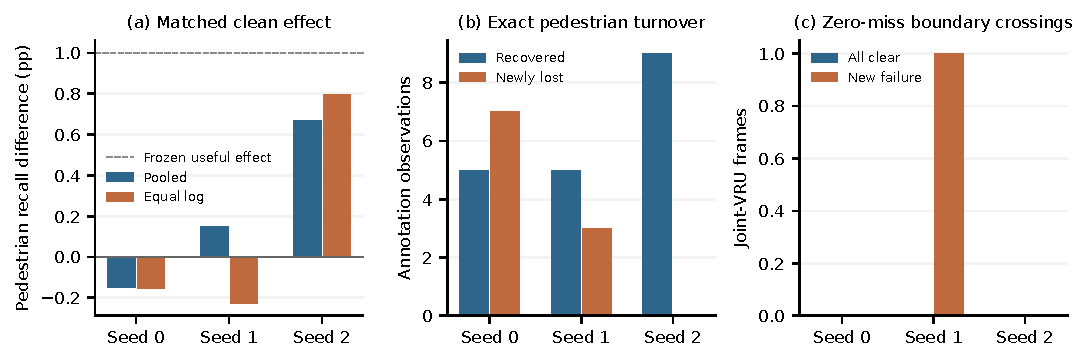
\includegraphics[width=\textwidth]{images/primary_identity_effects.pdf}
\caption{All three primary clean seeds: pooled and equal-log pedestrian effects, exact recovered/newly-lost annotation observations, and joint failed-frame changes. The same 162-frame historical panel is reused. Counts refer to matcher assignments, not distinct people or independently sampled frames.}\label{fig:primary}
\end{figure*}

The number of frames with improved pedestrian hit counts is three, four, and eight. Every such frame still misses at least one pedestrian. All five, five, and nine recovered pedestrian observations, respectively, occur on frames that remain joint failures, including recoveries in equal-count exchange frames. Seed~2 is especially instructive: nine recovered observations and no newly lost pedestrians improve recall, yet all nine occur on still-failed frames and AnyMiss remains unchanged. This is direct endpoint accounting, not evidence about the physical severity of those misses.

\begin{figure*}[t]
\centering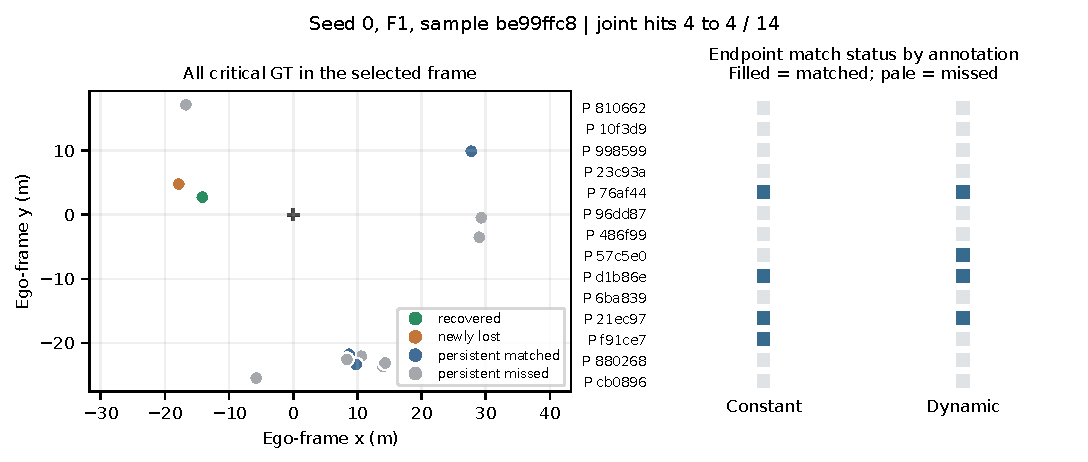
\includegraphics[width=0.96\textwidth]{images/identity_case.pdf}
\caption{Deterministically selected identity illustration: seed~0, clean F1 frame \texttt{be99ffc878b24aca8956bbb4e0f97d0c}. Among 14 critical pedestrian annotations, both arms match four and miss ten; one annotation is recovered and another newly lost. The left panel locates annotations in ego coordinates; the right panel shows the 14 matched-status assignments. P denotes pedestrian and suffixes abbreviate annotation IDs. Selection uses the first lexicographic qualifying frame with at most 20 targets, prioritizing equal-count identity exchange; it selects an illustration, not a model or outcome estimate. Colors encode the declared matcher, without image-based adjudication or cross-run prediction tracking.}\label{fig:case}
\end{figure*}

\subsection{Secondary views and the neutral parent}
% Generated from analysis/results.json SHA256 da5dbfb0c658a72ddddfcfc12c54ac1523bfc23094f806cef8627830b8c851da
% Generated from mechanism/RESULTS.json SHA256 3c491671a72237b819dfa725a969a978ade9430f347126e4bc921b0f9215186f
% Generated from mechanism/INFERENCE_GATE_STATISTICS.csv SHA256 445a4a298458eaf9d99f4981eca4be1b3ae5389261a8e0870aab6ee421249b43
% Generated from make_paper_tables.py SHA256 c0379ecdaac1296f16b841f096afbfa02ce6dc80253739e3b3da0d99554dfba0
\begin{table*}[t]
\centering
\footnotesize
\setlength{\tabcolsep}{3.5pt}
\caption{All fixed secondary dynamic-minus-constant views; SDK differences and pedestrian recall changes are pp. L50: outer LiDAR retention 0.5; Dec0: clean outer inference with decoder LiDAR input half zeroed; Dev: the original development roles, with different support shown explicitly. The support column is frames/pedestrian observations/joint-VRU observations. AnyMiss shows C$\to$D divided by target-containing frames, and burden is saved-pedestrian D/C. Dec0 is an inference intervention, not a retrained path-free comparison; Dev is descriptive and does not select checkpoints. These historically exposed, repeated seed populations are not independent data. NA denotes undefined, unavailable or unsupported values.}
\label{tab:new_secondary}
\begin{tabular}{ccrrrrrrr}
\toprule
View & Seed & Frames/Ped/Joint & $\Delta$ mAP & $\Delta$ NDS & $\Delta$ PedAP & $\Delta R_{\rm ped}$ & AnyMiss C$\to$D / N & Burden D/C \\
\midrule
L50 & 0 & 162/1347/1590 & +0.005 & -0.013 & +0.014 & -0.371 & $131\!\to\!131\;/\;137$ & 1.005 \\
L50 & 1 & 162/1347/1590 & +0.001 & +0.172 & -0.005 & +0.223 & $125\!\to\!124\;/\;137$ & 0.998 \\
L50 & 2 & 162/1347/1590 & -0.002 & +0.002 & +0.068 & +0.371 & $128\!\to\!127\;/\;137$ & 1.008 \\
Dec0 & 0 & 162/1347/1590 & -0.002 & +0.007 & +0.038 & -0.148 & $134\!\to\!134\;/\;137$ & 0.998 \\
Dec0 & 1 & 162/1347/1590 & -0.002 & +0.168 & +0.013 & +0.223 & $127\!\to\!127\;/\;137$ & 0.996 \\
Dec0 & 2 & 162/1347/1590 & 0.000 & +0.054 & +0.039 & +0.297 & $128\!\to\!128\;/\;137$ & 1.002 \\
Dev & 0 & 82/315/336 & +0.020 & +0.018 & -0.054 & -1.270 & $61\!\to\!61\;/\;65$ & 0.999 \\
Dev & 1 & 82/315/336 & +0.014 & -0.008 & +0.131 & +0.952 & $64\!\to\!64\;/\;65$ & 1.002 \\
Dev & 2 & 82/315/336 & +0.077 & +0.035 & +0.231 & 0.000 & $57\!\to\!57\;/\;65$ & 1.004 \\
\bottomrule
\end{tabular}
\end{table*}

Table~\ref{tab:new_secondary} preserves every fixed secondary row. Under 50\% LiDAR retention, the three pedestrian effects are $-0.371,+0.223,+0.371$ pp, with joint failure changes $0,-1,-1$. Decoder-half masking gives $-0.148,+0.223,+0.297$ pp and no dynamic--constant failure-count changes. Development effects are $-1.270,+0.952,0.000$ pp; none changes joint failure counts. These views were completed without adapting the schedule, gate, or checkpoint to their outcomes.

\begin{figure*}[t]
\centering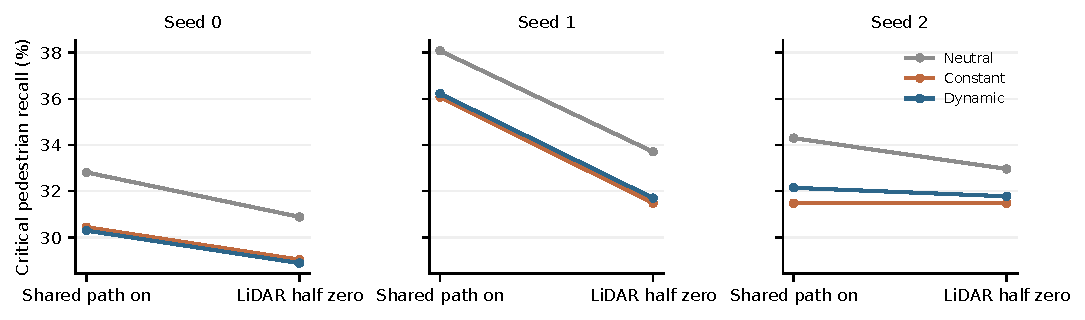
\includegraphics[width=\textwidth]{images/decoder_intervention.pdf}
\caption{Same-checkpoint decoder LiDAR input intervention for all evaluated clean arms and seeds. Encoder LiDAR remains enabled. Changes measure sensitivity to this masking operation on a detector trained with the route, not the effect of retraining without it or a decomposition of predictive contribution.}\label{fig:decoder}
\end{figure*}

Compared with its unadapted U8000 parent, each adapted arm has fewer primary pedestrian and joint hits and more joint failed frames (Table~\ref{tab:new_main_clean}). Saved outputs also decrease. This establishes no practical improvement over the inherited detector under the chosen short adaptation schedule. The neutral parent has zero new updates rather than 600; the comparison cannot isolate the gate, encoder adaptation, optimization schedule, or their interaction as the cause. Reduced output burden is not an official precision improvement.

\section{Observed gate and path behavior}
% Generated from analysis/results.json SHA256 da5dbfb0c658a72ddddfcfc12c54ac1523bfc23094f806cef8627830b8c851da
% Generated from mechanism/RESULTS.json SHA256 3c491671a72237b819dfa725a969a978ade9430f347126e4bc921b0f9215186f
% Generated from mechanism/INFERENCE_GATE_STATISTICS.csv SHA256 445a4a298458eaf9d99f4981eca4be1b3ae5389261a8e0870aab6ee421249b43
% Generated from make_paper_tables.py SHA256 c0379ecdaac1296f16b841f096afbfa02ce6dc80253739e3b3da0d99554dfba0
\begin{table*}[t]
\centering
\footnotesize
\setlength{\tabcolsep}{4.0pt}
\caption{Realized fixed-checkpoint gate behavior on clean outer frames, for every fold/seed. The dynamic SD column is the largest across-frame coefficient standard deviation among the four layers (pp), not variation across layers within one frame. Maximum baseline deviation is the largest absolute dynamic change (pp). Constant SD is defined identically. Boundary occupancy is the largest layer fraction (\%) at $\geq99\%$ of that layer's allowed amplitude. The absolute coefficient bound is at most 10 pp, reduced near probability boundaries. These are descriptions of historically exposed frames, not efficacy estimates or independent samples.}
\label{tab:new_mechanisms}
\begin{tabular}{ccrrrrr}
\toprule
Fold & Seed & Frames & Dynamic max SD (pp) & Max deviation (pp) & Constant max SD (pp) & Boundary occupancy (\%) \\
\midrule
F1 & 0 & 80 & 0.34008 & 2.015 & 0.00000 & 0.000 \\
F1 & 1 & 80 & 0.21272 & 1.356 & 0.00000 & 0.000 \\
F1 & 2 & 80 & 0.17068 & 1.734 & 0.00000 & 0.000 \\
F2 & 0 & 82 & 0.31229 & 1.844 & 0.00000 & 0.000 \\
F2 & 1 & 82 & 0.20672 & 1.130 & 0.00000 & 0.000 \\
F2 & 2 & 82 & 0.24261 & 2.633 & 0.00000 & 0.000 \\
\bottomrule
\end{tabular}
\end{table*}

Training telemetry agrees with neutral initialization: all twelve runs have positive first-update output-head gradient norms, while all 36 recorded descriptor/projection/hidden module groups have zero first-update gradients. Earlier module gradients subsequently become positive in all twelve runs. These observations verify that the intended learning paths activate; they do not establish useful conditioning.

At the fixed final checkpoints, the largest across-frame coefficient SD among four layers ranges from 0.17068 to 0.34008 pp over the six dynamic fold/seed models. The largest absolute departure from an inherited coefficient ranges from 1.130 to 2.633 pp. Constant descriptors yield zero across-frame coefficient SD. No recorded clean outer coefficient reaches 99\% of its allowed amplitude. The realized dynamic gate is therefore frame-dependent and remains well inside its bound on these frames; bound saturation does not describe the observed weak result. No matched unbounded experiment identifies what an alternative amplitude would do.

The same checkpoint produces identical coefficients before and after decoder-input masking because the intervention occurs downstream of gate computation. The recorded pre-mask encoder and decoder-LiDAR input norms establish that both inputs are present. LayerNorm scaling and norms are not calibrated contribution fractions: their magnitude cannot establish LiDAR dominance, gate redundancy, or causal responsibility. Masking changes detector outcomes, but a retrained route-free model could behave differently. The isolated all-camera-masks-empty forward check returns exactly $2q$ in evaluation; this narrowly verifies the audited branch and says nothing about its frequency or metric impact in the real panel.

\section{What the matched comparison resolves}
The direct dynamic--constant contrast removes the obvious static-four-logit versus MLP parameter-count difference from this new experiment, while retaining common feature pooling, initialization, draws, updates, and decoder paths. It strengthens the interpretation of a conditioning comparison under the specified bounded parameterization. It does not retrospectively show that earlier gains were capacity artifacts: the predecessor already included the same-sized A3 control, and this study changes the panel and residual formula.

The results distinguish three statements. First, the gate learns and responds to frames; the gradient and fixed-checkpoint variation records support that implementation statement. Second, a few annotations change from missed to matched, with small and seed-dependent net changes. Third, the practical criterion is not met: no primary seed obtains the minimum recall increase, and the positive pooled seed~1 effect accompanies negative equal-log recall and an additional failed frame. Evidence for the first two statements cannot be substituted for the third.

A scalar per layer aggregates detection gradients over a whole frame. The observed combination of recoveries and persistent failures is compatible with that architecture, but this experiment does not establish the mechanism causing any particular annotation to recover. Recoveries on already failed frames explain the arithmetic gap between count recall and AnyMiss; they do not show that the recovered objects are unimportant. A useful next hypothesis would require its own frozen design, new evidence, and explicit budget. No such expansion is executed here after failure of the current screen.

\section{Limits of interpretation}
Historical mini exposure, repeated instances, few logs, overlapping folds, short adaptation, inherited detector quality, and the shared decoder path restrict interpretation. Freezing a new protocol does not erase previous selection or inspection; finite-sample selection bias remains relevant~\cite{Cawley2010Selection}. Three seeds reuse the same data and are not independent datasets. We report no iid-frame confidence intervals, $p$-values, causal effects, safety calibration, collision-risk reduction, SOTA result, or external generalization. An unsuccessful matched comparison can establish a useful boundary for this implementation, but not the impossibility of conditional fusion. Original failures, missingness, conditional stops, and the original \texttt{NO\_PROMOTION} decision remain preserved. Code development used AI assistance.

The new annotation identities describe assignments under the declared greedy matcher. They are not visual adjudication or proof of unique-person recovery, and they do not repair identities missing from old experiments. No matched unbounded gate or retrained path-free detector is included. Checkpoint-availability-based panel choice is not random sampling of capture logs. Parents and backbone strategies remain products of the historically inspected original procedure; final-step reuse does not remove their earlier development exposure. New detector outputs also prevent transfer of the old monitor's scores or claims; monitoring efficacy for these new boxes is not evaluated.

\section{Verification, cost, and availability}
The protocol hash begins \texttt{b368607bb33f}; the pre-compute freeze manifest begins \texttt{125fb0f61d6b}. Full hashes bind consumed source, configuration, metadata, parent checkpoints, and newly saved prediction/identity files. Runtime guards record matching inherited initialization, actual paired sample sequences, and equality of frozen/shared tensors. A separate standard-library verifier checks those saved receipts and checkpoint byte hashes; it does not independently reload and compare all PyTorch tensors.

Completed new work comprises 7,200 scientific and three engineering optimizer updates, with no scientific retries, failed scientific trajectories, or unknown optimizer starts. Conservative single-GPU reserved time is 5,175.72 seconds (1.438 hours), including engineering, inference, CPU work and I/O inside those actions; inherited U8000 training is excluded from new cost. The first-to-last compute span is 5,306.05 seconds. Subsequent 108-call per-log SDK aggregation uses no model or new inference and takes 265.86 wall seconds (263.08 process CPU seconds). CPU analysis, document preparation and backup are separate from GPU-reserved time. The declared 12-run and compute ceilings are not expanded following the result.

Numerical verification passes 9,042,589 scalar checks across all sixty evaluation groups, including count identities, sample unions, paired receipts, completed updates, costs, and 39 comparisons. A separate class-separated greedy reconstruction independently rebuilds every eligible ground-truth assignment from saved predictions in all sixty groups, with zero identity discrepancies or numerical ambiguities. It includes targets outside the critical region before applying the endpoint restriction. These are independent implementations within the same AI-assisted workflow, not an independent laboratory or fresh-data replication.

The English public companion is available at \url{https://github.com/xiaotwu/layergate-bev-critical-miss-evaluation}. It preserves the earlier report and adds this paper, LaTeX, one-page summary, portable protocol, all primary and secondary aggregate results, exact critical matching-status records, per-log SDK/support records, gate source, checksums, and a standard-library compact reproduction script. Its compact verification performs 202,056 checks over saved matching-status/count/decomposition/criterion records and synthetic contracts across thirty pooled scopes and 39 comparisons, plus 39 manifest-file checks (202,095 total in the default command). It does not rematch boxes, run a detector, recompute official SDK metrics, or reproduce training from that compact package. SDK values and norm telemetry are labeled copied outputs. Full local new-run checkpoints, prediction files, logs, source and verification receipts are retained in an incremental, hash-verified backup. Dataset and upstream-code terms remain applicable; no sensor data, parent checkpoints, or third-party LaTeX class are redistributed.

\section{Conclusion}
The bounded frame-conditioned gate is operational, but its matched comparison does not meet the frozen useful-effect criterion on the four-log mini panel. Small observation-level recoveries coexist with new losses, persistent failed frames, and heterogeneous log effects. Neither additional updates nor the shared decoder route can be assigned causal responsibility from this design. The appropriate completed outcome is a negative practical screen with mixed descriptive changes, preserved identities and costs, and no candidate expansion or promotion claim.
\bibliographystyle{IEEEtran}
\bibliography{references}
\end{document}
